\documentclass{article}

\usepackage{graphicx}
\usepackage{tikz}
\usepackage{tikzsymbols}
\usetikzlibrary{calc,patterns,shapes.geometric}
\pagestyle{empty}
\usepackage[margin=0pt]{geometry}
\geometry{papersize={14in,12in}}

\def\centerarc[#1](#2)(#3:#4:#5){\draw[#1] ($(#2)+({#5*cos(#3)},{#5*sin(#3)})$) arc (#3:#4:#5);}

\begin{document}
	\begin{figure}
		\centering
		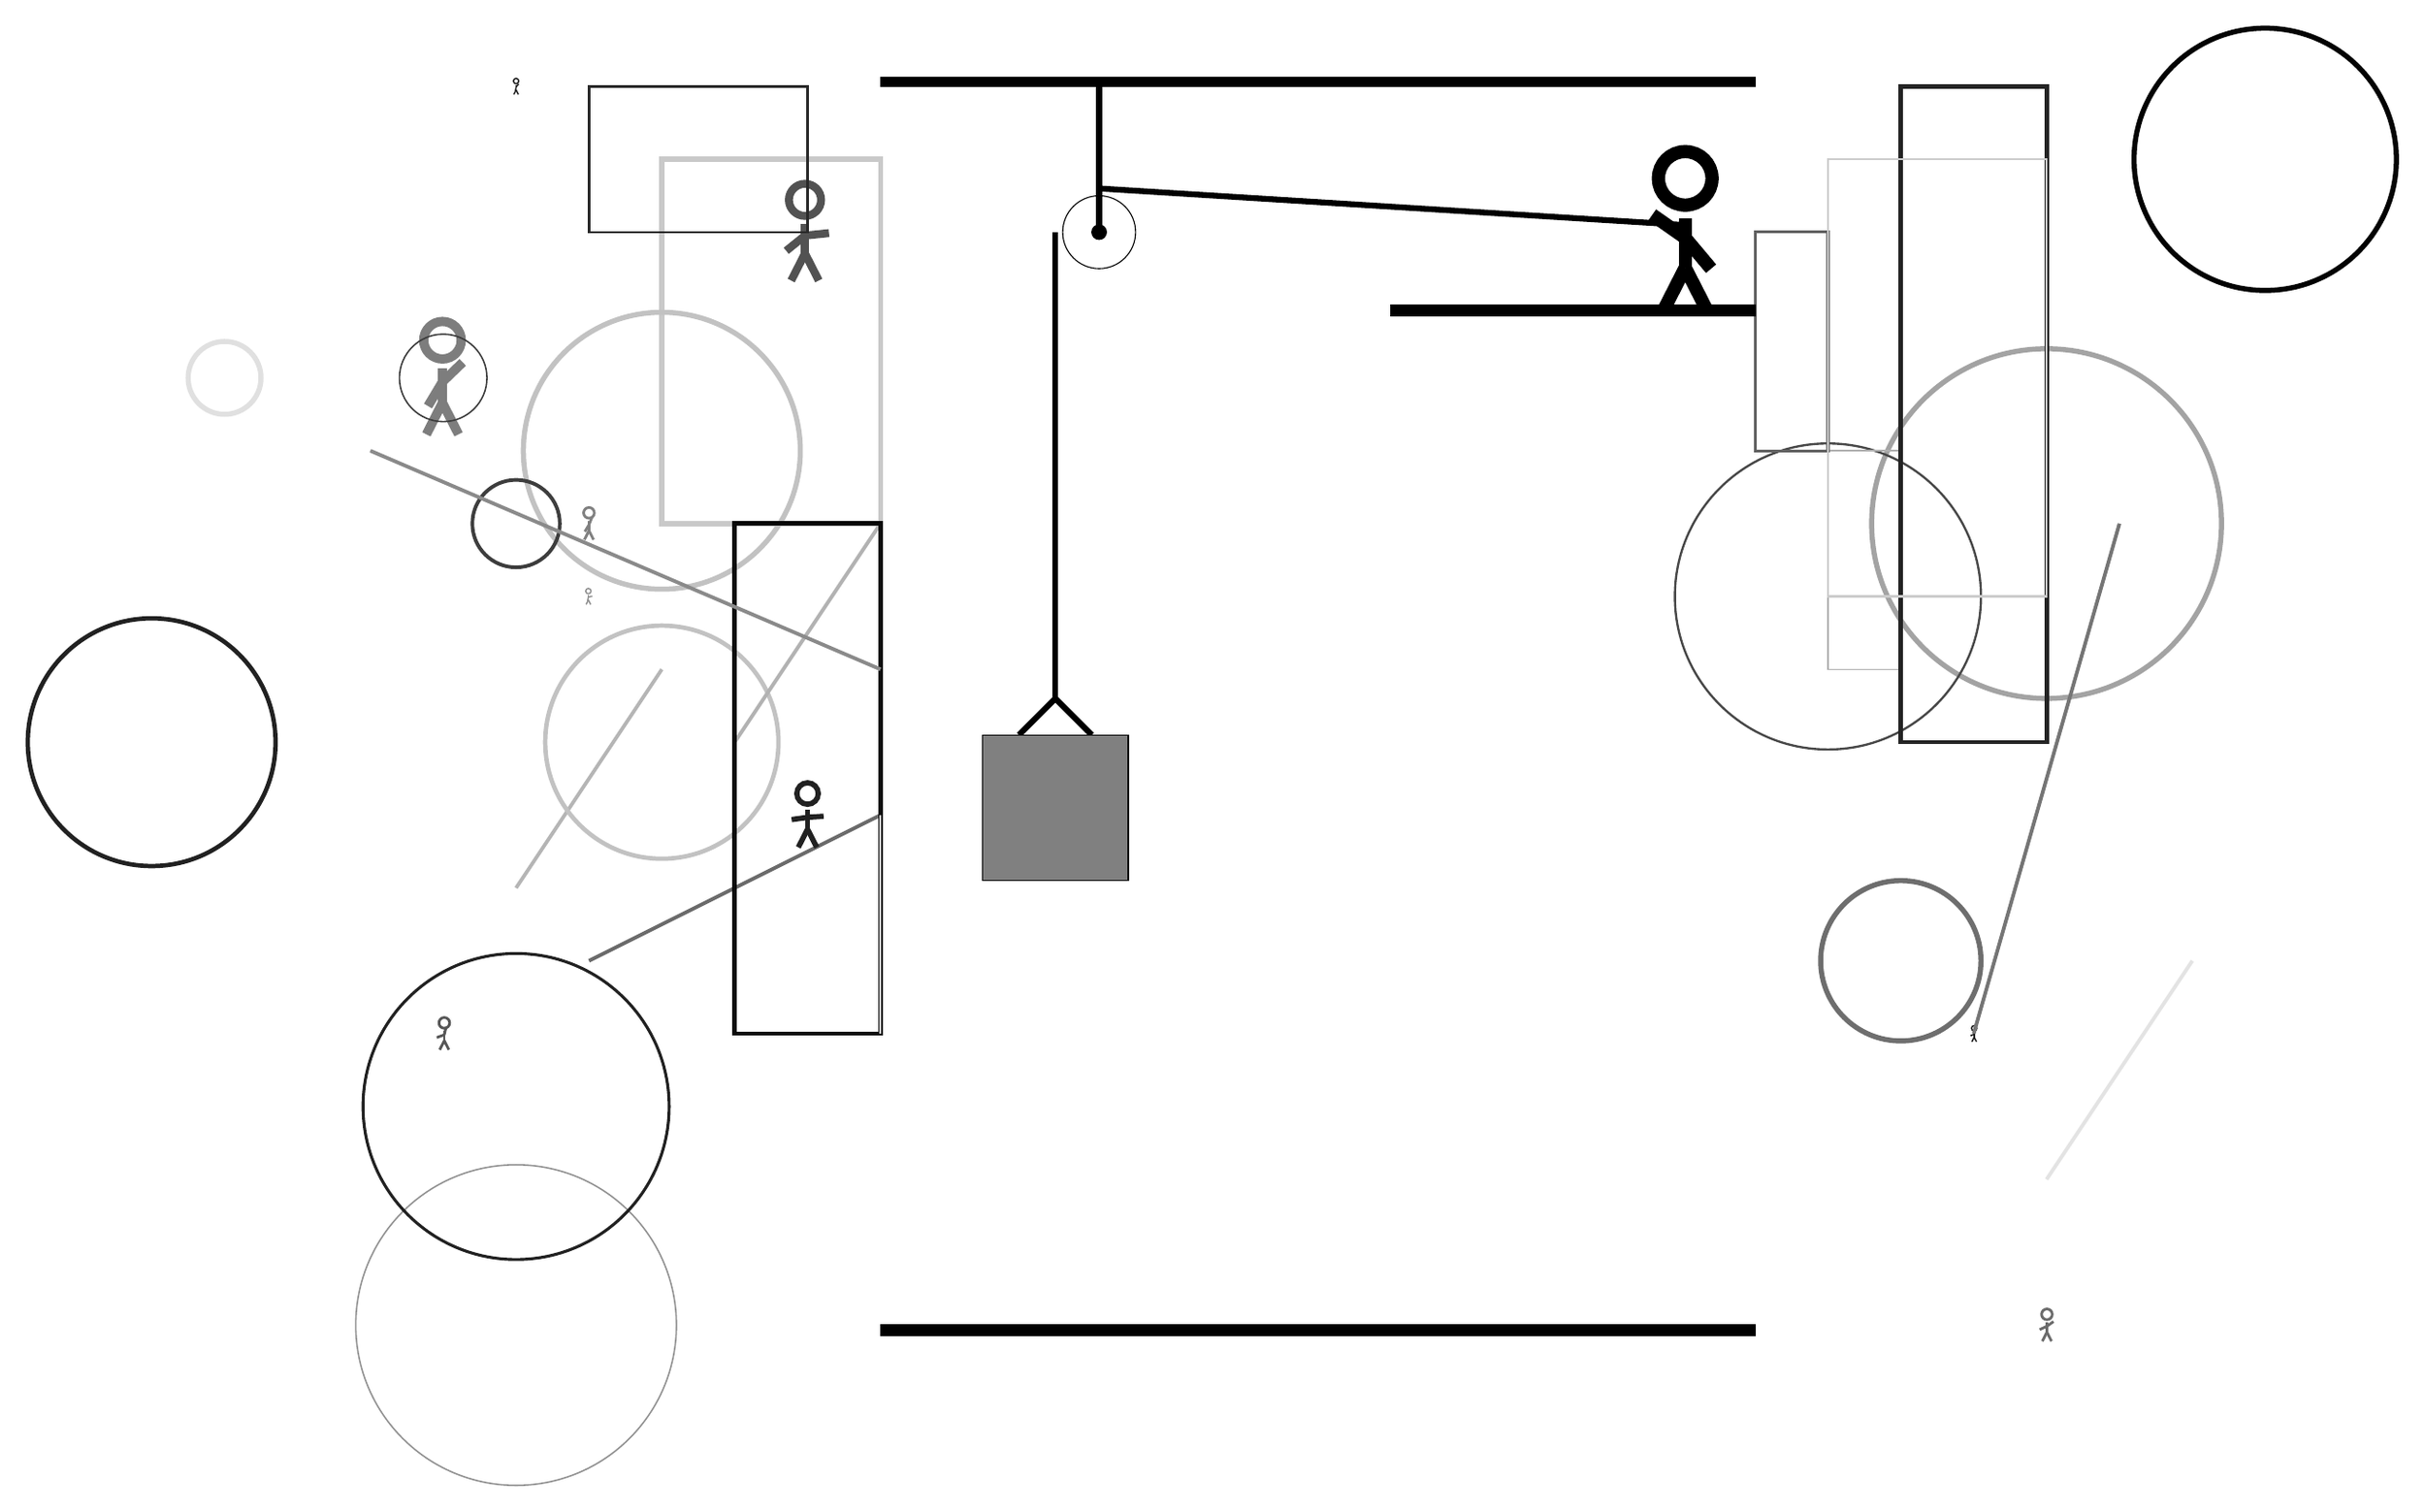
\begin{tikzpicture}
			%%%%% START %%%%%
			
			\draw[fill=black] (-2, 14) rectangle (10, 14.125);
			
			\draw (1, 12) circle (0.5);
			\draw[fill=black] (1, 12) circle (0.1);
			\draw[line width=0.8mm] (1, 14) -- (1, 12);
			
			\draw[line width=0.8mm](-0.1, 5.1) --  (0.4, 5.6) -- (0.9, 5.1);
			\draw[fill=black!50] (-0.6, 5.1) rectangle (1.4, 3.1);
			
			\draw [line width=0.7mm, color=black!36](14, 8) circle (2.4);
			
			\draw[line width=0.7mm, color=black!21] (-2, 8) rectangle (-5, 13);
			\draw [line width=0.7mm, color=black!12](-11, 10) circle (0.5);
			\node[line width=0.2mm, color=black!89] at (-7, 14) {\Strichmaxerl[1][81][51]};
			\draw [line width=0.3mm, color=black!72](11, 7) circle (2.1);
			\node[line width=0.5mm, color=black!68] at (-3, 12) {\Strichmaxerl[6][39][6]};
			\draw[line width=0.5mm, color=black!11](14, -1) -- (16, 2);
			\draw[line width=0.2mm, color=black!31] (12, 9) rectangle (11, 6);
			\draw[line width=0.5mm, color=black!58](-2, 4) -- (-6, 2);
			\draw [line width=0.7mm, color=black!24](-5, 9) circle (1.9);
			
			\draw[line width=0.3mm, color=black!84] (-3, 14) rectangle (-6, 12);
			\node[line width=0.4mm, color=black!87] at (-3, 4) {\Strichmaxerl[4][8][4]};
			\draw[line width=0.6mm, color=black!86] (12, 14) rectangle (14, 5);
			\draw[line width=0.5mm, color=black!29](-5, 6) -- (-7, 3);
			\draw [line width=0.6mm, color=black!24](-5, 5) circle (1.6);
			\node[line width=0.2mm, color=black!58] at (14, -3) {\Strichmaxerl[2][25][35]};
			
			\draw[line width=0.4mm, color=black!62] (10, 9) rectangle (11, 12);
			
			\draw[line width=0.3mm, color=black!20] (11, 13) rectangle (14, 7);
			\node[line width=0.7mm, color=black!91] at (13, 1) {\Strichmaxerl[1][22][76]};
			
			\draw[line width=0.5mm, color=black!54](13, 1) -- (15, 8);
			\node[line width=0.3mm, color=black!50] at (-6, 8) {\Strichmaxerl[2][59][68]};
			
			\node[line width=0.7mm, color=black!51] at (-8, 10) {\Strichmaxerl[7][59][44]};
			\draw[line width=0.5mm, color=black!30](-2, 8) -- (-4, 5);
			\draw [line width=0.2mm, color=black!77](-8, 10) circle (0.6);
			\draw[line width=0.6mm, color=black!96] (-2, 8) rectangle (-4, 1);
			
			\draw [line width=0.7mm, color=black!57](12, 2) circle (1.1);
			\draw [line width=0.5mm, color=black!76](-7, 8) circle (0.6);
			\draw [line width=0.2mm, color=black!43](-7, -3) circle (2.2);
			\draw[line width=0.3mm, color=black!11] (-2, 1) rectangle (-2, 4);
			\node[line width=0.3mm, color=black!44] at (-6, 7) {\Strichmaxerl[1][79][11]};
			\node[line width=0.5mm, color=black!66] at (-8, 1) {\Strichmaxerl[2][20][77]};
			
			\draw [line width=0.7mm, color=black!99](17, 13) circle (1.8);
			\draw[line width=0.5mm, color=black!46](-2, 6) -- (-9, 9);
			\draw [line width=0.6mm, color=black!87](-12, 5) circle (1.7);
			
			\draw [line width=0.4mm, color=black!87](-7, 0) circle (2.1);
			
			\draw[line width=0.8mm](0.4, 12) -- (0.4, 5.6);
			\centerarc[line width=0.8mm](1, 12)(90:180:0.6)
			\draw[line width=0.8mm](1, 12.6) -- (9, 12.1);
			
			\node at (9, 12) {\Strichmaxerl[10][-35][-50]};
			\draw[fill=black] (5, 11) rectangle (10, 10.85);
			
			\draw[fill=black] (-2, -3) rectangle (10, -3.15);
			
			%%%%% END %%%%%
		\end{tikzpicture}
	\end{figure}	
\end{document}